\section{Das Potenzial-Problem}

\subsection{Spezialfall k = 1}
//algo angeben, wieso ist er liniear? wieso korrekt?\\


Die Idee des Algorithmus ist es, zu protokollieren, welche Kante(n) für welche Knoten von Bedeutung ist:\\

Jeder Knoten berechnet im Algorithmus von BARRIÈRE L. et al. die minimale Anzahl von Agenten und jede Knoten hat mindestens eine Kante von der seine Agentenanzahl von abhängt.

\subsection{Potenzial auf einer Kante mit k > 1}

Um das Problem des Potenzials etwas zu erweitern, betrachte ich im folgenden Abschnitt Potenziale größer 1, allerdings mit der Einschränkung, dass man das gesamte Potenzial k nur auf einer Kante einsetzen darf.

Es fällt zunächst auf, dass man nicht garantieren kann, dass sich die Anzahl der benötigten Agenten auf allen Bäumen reduzieren lässt. Hierbei spielt es auch keine Rolle, wie groß das Potenzial k ist, da allein die Eigenschaft, dass man das Potenzial nur auf einer Kante einsetzen kann, genügt, um ein Gegenbeispiel zu finden:

Da das Potenzial k beliebig groß ist, kann man eine Kante auf Kantengewicht 1 setzen, man dadurch das größtmögliche Potenzial ausnutzt. Trotzdem ist es nicht möglich bei folgendem Baum die Anzahl der Agenten zu reduzieren:

\begin{figure}[h]
	\subfigure[alle Kanten haben Gewicht 4. Alle Knoten benötigen mindestens 8 Agenten.]{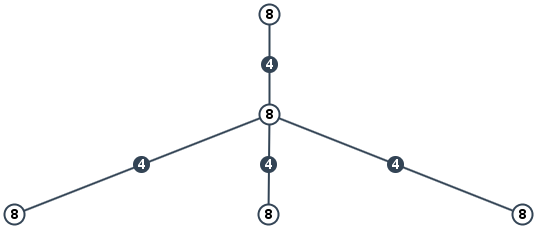
\includegraphics[width=0.49\textwidth]{bilder/abb1.png}} 
	\subfigure[eine Kante wurde auf Gewicht 1 geduziert, alle anderen haben weiterhin Gewicht 4. Alle Knoten benötigen trotzdem mindestens 8 Agenten.]{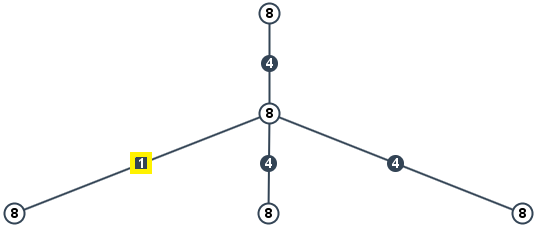
\includegraphics[width=0.49\textwidth]{bilder/abb2.png}} 
	\caption{Beispiel, dass Verringerung auf einer Kante nicht zu einer Verringerung der notwendigen Agenten führen muss} 
\end{figure} 

TODO:\\
//überlegung: woran sieht man, ob man die Agentenanzahl verringern kann?\\
//algorithmus angeben, welche kante ausgesucht wird?\\

\subsection{Potenzial verteilen mit k > 1}